% !TeX root=main.tex
\pagenumbering{arabic}
\chapter{تعریف مسئله}
\thispagestyle{empty}

تشخیص موضع در مطالعات تحلیلی برای تشخیص جهت گیری افکار عمومی در رسانه‌های اجتماعی، مانند مسائل سیاسی و اجتماعی، نقش کلیدی ایفا می‌کند. از این رو می‌تواند در شبکە‌های اجتماعی در بستر اهداف مختلفی از جمله تصمیمات دولت، تبلیغات، اقناع افکار عمومی مورد استفاده قرار بگیرد. به عبارتی دیگر نتایج به دست آمده منجر به دید وسیع تری به نظرات عمومی و اخذ تصمیمات بهتر می‌شود.


\section{سطوح مسئله تشخیص موضع}\label{sec:stance-detection-level}
قبل از بررسی گونە‌های مختلف تشخیص موضع، شناخت دقیق سطوح مختلف تشخیص موضع از اهمیت
بالایی برخوردار است. مسئله تشخیص موضع معمولا در دو سطح بررسی می‌شود. در ادامه توضیحات
مختصری از این دو سطح را بیان می‌شود.
\begin{enumerate}
	\item 
	 سطح بیانیه
	 \LTRfootnote{\lr{The Statement Level}}
	\newline
در این سطح هدف این است موضع یک متن نوشته شده نسبت به موضوع از قبل مشخص شده،
تعیین گردد. این سطح معمول‌ترین روش به کارگرفته شده در تشخیص موضع است. به صورتی که
ویژگی‌‌های متن نوشته شده استخراج می‌شود و تشخیص موضع صرفا بر اساس متن انجام می‌شود. این مفهوم معمولا به صورت ردە‌بندی با سه کلاس (موافق، مخالف، بدون نظر) تعریف می‌شود.  بدون نظر یعنی متن نوشته شده نسبت به موضوع بی ربط است. حالت دیگر این است که موضوع در
آن بررسی شده ولی موضع مشخصی در رابطه با آن (موافق یا مخالف) ندارد.
	\item  سطح کاربر
	\LTRfootnote{\lr{The User Level}}
	
در این سطح هدف پیشبینی موضع کاربر نسبت به یک موضوع می‌باشد. متغیرهای مختلفی که
یک کاربر از خود در شبکه‌‌های اجتماعی به جای می‌گذارد، در بررسی‌‌ها مورد استفاده قرار می‌گیرد.
پست‌های کاربر، پست‌هایی که پسندیده و یا مجدد به اشتراک گذاشته، از جمله اطلاعاتی‌ است که در این فرآیند مورد استفاده قرار می‌گیرد. در این سطح معمولا ردە بندی با دو کلاس (موافق و مخالف) تعریف می‌شود. چرا که این فرض در نظر گرفته شده که حتی اگر بعضی از پست‌های کاربر در رابطه با موضوع معین بدون موضع باشد، اما به هر حال کاربر یک موضع مشخصی نسبت به آن موضوع دارد.

\end{enumerate}

آشنایی با سطوح مختلف تشخیص موضع و تفاوت آن‌ها بسیار با اهمیت است. پست‌های مختلف یک کاربر نسبت به یک موضوع می‌تواند موضع‌های مختلفی داشته باشد. ولی‌ زمانی که در سطح کاربر مسئله تشخیص موضع را تعریف می‌کنیم، موضع کلی کاربر نسبت به موضوع مطرح می‌شود.

\section{تقسیم بندی تشخیص موضع بر اساس موضوع}
در تشخیص موضع همان‌طور که در گذشته بیان کردیم، نیاز به مشخص بودن یک موضوع (هدف) برای تشخیص موضع در رابطه با آن وجود دارد.

\subsection[تشخیص موضع برای یک موضوع خاص]{تشخیص موضع برای یک موضوع خاص\LTRfootnote{\lr{Target-specific Stance Detection}}
}
رایج ترین نوع تشخیص موضع در شبکه‌های اجتماعی، تشخیص موضع برای یک موضوع خاص است. در
این نوع تشخیص موضع متن یا کاربر، ورودی اصلی برای پیش‌بینی موضع نسبت به یک هدف مشخص است. بنابراین برای هر هدف یک مدل ردە‌بندی جداگانه آموزش داده می‌شود.

\subsection[تشخیص موضع برای موضوعات چندگانه مرتبط]{تشخیص موضع برای موضوعات چندگانه مرتبط\LTRfootnote{\lr{Multi-Related-Target Stance Detection}}}
در این روش، تشخیص موضع نسبت به چندین هدف مرتبط انجام می‌شود. این هدف‌ها می‌توانند یک موضوع کلی، رویداد خاص و یا اشخاص مختلف باشند. دادە‌های یک هدف می‌تواند دانشی برای هدف‌های دیگر داشته باشد. به عنوان مثال فردی که موافقت خود را با یکی از نامزدهای انتخابات ریاست جمهوری اعلام می‌کند، به صورت متوالی مخالف خود را با نامزد حزب (گروه) مقابل نیز اعلام کرده است.

لازم به ذکر است نوع دیگری از تشخیص موضع با عنوان تشخیص موضع برای موضوع متقابل
\LTRfootnote{\lr{Cross-Target Stance Detection}}
نیز تعریف شده است. در این روش آموزش مدل بر روی یک موضوع مشخص انجام می‌شود. در مرحله ارزیابی دادە‌های موضوع متفاوت اما مرتبط با موضوع زمان آموزش مورد استفاده قرار می‌گیرد. در شرایطی که مجموعه داده کافی برای آموزش مدل با بهترین عملکرد در دسترس نباشد، یکی از ایدە‌های قابل استفاده این مورد می‌باشد. به عنوان مثال در پژوهش 
\cite{xu-etal-2018-cross}
آموزش مدل بر روی دادە‌ها با برچسب هیلاری کلینتون انجام می‌شود. در زمان ارزیابی از دادە‌ها با برچسب دونالد ترامپ استفاده می‌شود. در واقع همچون حالت قبل مدل
به نوعی آموزش می‌بیند که بتواند برای دو موضوع متفاوت ولی مرتبط عملیات تشخیص موضع را انجام دهد.

\subsection[تشخیص موضع ادعا محور]{تشخیص موضع ادعا محور
\LTRfootnote{\lr{Claim-Based Stance Detection}}}
در این حالت هدف تشخیص موضع، یک هدف مشخص (صریح) مثل شخص، رویداد نیست. در واقع هدف
در اینجا می‌تواند ادعای عنوان خبر یا شایعه باشد. در ادامه برای آشنایی بیشتر با مسائل مرتبط و فهم جایگاه مسئله اصلی، توضیح دقیق‌تر انواع آن و برچسب‌های موجود در هر مورد را بررسی می‌کنیم.
\begin{enumerate}
	\item  
	تشخیص موضع در اخبار جعلی
	\LTRfootnote{\lr{Fake News Stance Detection}}
	\newline
	در این حالت ورودی تیتر خبر
	\LTRfootnote{\lr{News Headline}}
	به همراه یک متن خبری کامل
	\LTRfootnote{\lr{News Body}}
	می‌باشد (تیتر خبر و متن خبر ممکن است برای دو خبر کاملا متفاوت باشند). در نهایت هدف این است موضع متن خبری نسبت به ادعا مطرح شده در تیتر خبر مورد بررسی قرار بگیرد. این مسئله به صورت ردە‌بندی با‌ چهار کلاس (تایید‍~
			\LTRfootnote{\lr{Agrees}}، رد
			\LTRfootnote{\lr{Disagrees}}
	، بحث شده (موضوع مرتبط بدون نظر قطعی)
			\LTRfootnote{\lr{Discusses}}
	، نامرتبط
			\LTRfootnote{\lr{Unrelated}}
	) تعریف می‌‌شود. این مسئله برای حل تشخیص اخبار جعلی مطرح می‌شود.
	\item 
	تشخیص شایعه
	\LTRfootnote{\lr{Rumer Stance Detection}}
	\newline
	در این حالت ورودی شایعه به همراه یک قطعه متن است. هدف این است موضع نویسنده متن نسبت به صحت شایعه مطرح شده سنجیده شود. این مسئله به صورت ردە‌بندی تعریف می‌شود. در بعضی تعاریف ردە‌بندی با چهار کلاس شامل (تایید
		\LTRfootnote{\lr{Supporting}}
	، رد
		\LTRfootnote{\lr{Denying}}
	، پرس و جو
			\LTRfootnote{\lr{Querying}}
	 و اظهارنظر
	 		\LTRfootnote{\lr{Commenting}}
	 ) تعریف می‌شود. در برخی دیگر از تعاریف ردە‌بندی با دو کلاس (تایید
		\LTRfootnote{\lr{Supporting}}
	 و رد
	 	\LTRfootnote{\lr{Denying}}
	 ) تعریف می‌شود.
\end{enumerate}
\subsection{تفاوت تشخیص موضع و تحلیل احساسات}
مسئله تحلیل احساسات
	\LTRfootnote{\lr{Sentiment Analysis}}
	به عنوان مسئله پردازش احساسی متون در نظر گرفته می‌شود که می‌تواند بدون
	داشتن یک هدف مشخص استنباط شود. در این مسئله مشخص می‌شود یک متن نوشته شده بر اساس محتوای زبان، احساس مثبت
		\LTRfootnote{\lr{Positive}}،
		منفی
		\LTRfootnote{\lr{Negative}}
			یا خنثی
		\LTRfootnote{\lr{Neutral Sentiment}}
				دارد.  در حالی که در تشخیص موضع موافق یا مخالف بودن
			نویسنده متن با موضوع مشخص شده، مد نظر است. شکل
			\ref{sem-eval-label}
توزیع برچسب‌های تحلیل احساسات نسبت به تشخیص موضع در مجموعه داده
			 \lr{SEM-Eval2016}
			\cite{Sobhani2016DetectingSI}
را نشان می‌دهد. برچسب‌های تحلیل احساسات و تشخیص موضع همیشه یکسان نیست. به عنوان مثال تمام دادگانی که در تحلیل احساسات برچسب مثبت دارند، در تشخیص موضع برچسب موافق نگرفتە‌اند. حدود ۳۰ درصد موافق و حدود ۳۳ درصد مخالف و مابقی نیز برچسب خنثی دارند.
\begin{figure}[H]
	\vspace{-0.5cm}
	\center{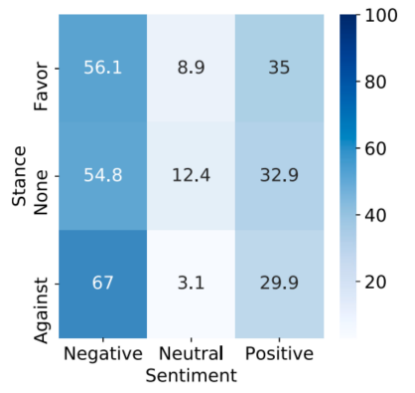
\includegraphics[width=0.4\linewidth]{images/sem-eval-label.PNG}}
	\caption[توزیع برچسب‌های تحلیل احساسات نسبت به برچسب‌های تشخیص موضع]{توزیع برچسب‌های تحلیل احساسات نسبت به برچسب‌های تشخیص موضع در مجموعه دادگان
	\lr{SEM-Eval2016} \cite{ALDAYEL2021102597}\label{sem-eval-label}}
	
\end{figure}	



\begin{table}[h!]
\caption[نمونه‌ای از مجموعه داده
	\lr{SemEval}]{نمونه‌ای از مجموعه داده
\lr{SemEval}\cite{ALDAYEL2021102597}\label{example}}
	\centering
	\begin{tabular}{c  c c c}

		متن توییت & موضوع & تشخیص موضع & تحلیل احساسات
		\\
		\hline
	
				\begin{tabular}{@{}c@{}}
						\lr{I am sad that Hillary lost} \\ 
						\lr{this presidential race.}\\
			    \end{tabular}
				 & \lr{Hillary Clinton} & موافق & منفی
		\\
		\hline
	\end{tabular}

\end{table}
به عنوان مثال و برای درک بهتر جمله و هدف حدول
\ref{example}
 را در نظر بگیرید 
\cite{mohammad-etal-2016-semeval}.
نویسنده متن، با متن نوشته شده نشان می‌دهد با کلینتون موافق است. در حالی‌ که از نظر احساسات، متن احساس منفی منتقل می‌کند. بنابراین می‌توان نتیجه گرفت دو مسئله تحلیل احساسات و تشخیص موضع به هم مرتبط هستند اما یکسان
نیستند 
\cite{Sobhani2016DetectingSI}.

پس به طور خلاصه دو تفاوت عمده مسئله تشخیص موضع و تحلیل احساسات شامل موارد زیر می‌شود. (۱)در تشخیص موضع، موضوع که نسبت به آن بررسی‌ها انجام می‌شود به طور کامل مشخص است. (۲)مانند مثال بالا برچسب‌های نهایی این دو مسئله می‌توانند کاملا با هم متفاوت باشد. بنابراین تفاوت این دو	مسئله کاملا مشهود است.

تحلیل احساسات جنبه گرا
	\LTRfootnote{\lr{Aspect-Oriented Sentiment Analysis}}
شبیە ترین مسئله موجود به تشخیص موضع می‌باشد. در این نوع از تحلیل احساسات موضوع معمولا شامل محصولات الکترونیکی(لپتاپ)، رستوران و هتل می‌باشد. جنبە‌های مورد بررسی نیز شامل قیمت، کیفیت، طرح می‌باشد. تفاوت تحلیل احساسات جنبه‌گرا با تشخیص موضع در این است که در تحلیل احساسات موضوعی که مورد بررسی قرار می‌گیرد در متن به صورت دقیق ذکر شده است. اما در تشخیص موضع لزوما این طور نیست. همچنین موضوع مورد بررسی در تشخیص موضع می‌تواند یک رویداد باشد ولی در تحلیل احساسات جنبە‌گرا این طور نیست.

\begin{figure}[H]
	\center{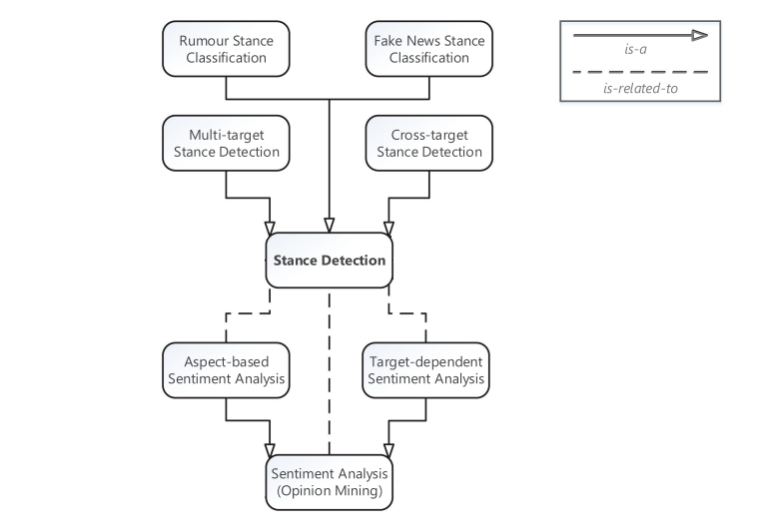
\includegraphics[width=0.8\linewidth]{images/stance_related_research.PNG}}
	\caption[موضوعات تحقیقاتی مرتبط با تشخیص موضع]{
		موضوعات تحقیقاتی مرتبط با تشخیص موضع
		 \cite{10.1145/3369026}\label{stance_related_research}}
	
\end{figure}

\subsection{کاربردهای تشخیص موضع}
بعد از مطرح شدن تعاریف مختلف مسئله تشخیص موضع، حال به بررسی تعدادی از کاربردهای مطرح شده می‌پردازیم. در مسئله تشخیص موضع، نظر و موضع افراد نسبت به هدف یا موضوع خاص سنجیده می‌شود. با توجه به این تعریف کابردهای زیر مطرح می‌شود.
\begin{enumerate}
	\item 
	 نظرسنجی و بررسی افکار عمومی: مطالعات تشخیص موضع معمولا بر روی محتوا آنلاین انجام می‌شود که موضوع آن مشخص است. از این رو با استفاده از تشخیص موضع خودکار، موافقت یا مخالف عموم افراد جامعه نسبت به موضوع خاصی را می‌توان ارزیابی کرد. این روش می‌تواند جایگزین نظرسنجی‌های سنتی باشد.
	 
	 \item 
	  سیستم‌های توصیە‌گر: در صورتی که موضع افراد نسبت به هدف و موضوعی معین را بدانیم، توصیه کردن محصولات به سادیگی میسر می‌شود.
	 \item 
	 
	 تبلیغات هدفمند: آگاهی از موضع کابران باعث می‌شود تبلیغات به صورت موثر و هدفمند انجام شود.

	 \item
	 
	 تشخیص اخبار جعلی 
	 \cite{popat-etal-2018-declare}
	 و تشخیص شایعه نیز از دیگر کابردهای قابل تعریف به کمک مسئله تشخیص موضع می‌باشند. در این مسائل معمولا از تشخیص موضع ادعا محور استفاده می‌شود.
	 				
\end{enumerate}


